
\chapter{RELATED THEORY}
\section{Microphone}
A microphone is a device that translates sound vibrations into electrical signals. It enables users to capture audio and transmit it to various devices such as recording medium or over a loudspeaker. Microphones are used in many applications such as telephones, sound engineering, live and recorded audio engineering, radio and television broadcasting, etc., for communication purposes.	 
\section{Arduino Nano}
\begin{figure}[h]
\centering  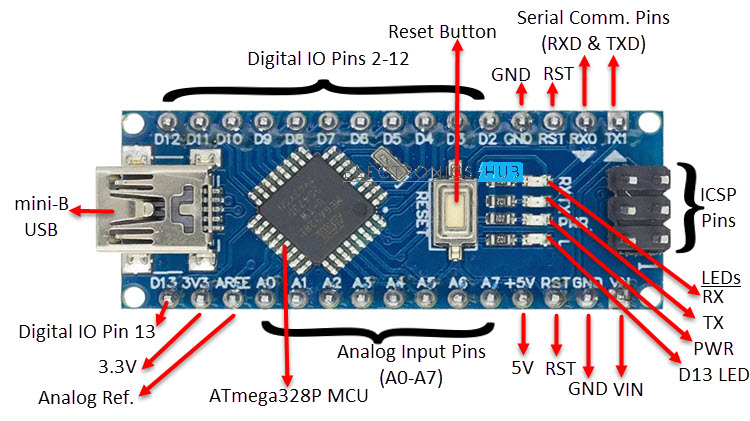
\includegraphics[width=0.5\textwidth]{Arduino Nano}
\caption{Arduino Nano}\\ 
Source: \textit{https://tinyurl.com/4hmte6dw}
\label{fig:ArduinoNano}
\end{figure}
The Arduino Nano is a small, breadboard-friendly microcontroller board based on the ATmega328. It is equipped with 30 male I/O headers which can be programmed using the Arduino Software IDE (Integrated Development Environment). It can communicate with a computer and other microcontrollers.It consists of flash memory  of 32KB capacity of which 2 KB is used for Bootloader.It supports Inter-Integrated Circuit (I2C), Serial Peripheral Interface (SPI) and Universal Asynchronous Receiver / Transmitter (UART).It has 10 bit ADC. 


\section{Raspberry Pi 4 Model B}
The Raspberry Pi is a credit card-sized single-board computer that provides a powerful processing platform in a compact form factor. It is equipped with a range of input/output interfaces, including USB ports, HDMI, Ethernet, GPIO (General Purpose Input/output), and a camera interface. The processor speed of Raspberry Pi 4 Model B is 1.5 GHz. It comes with onboard wireless networking and bluetooth.
\begin{figure}[h]
\centering  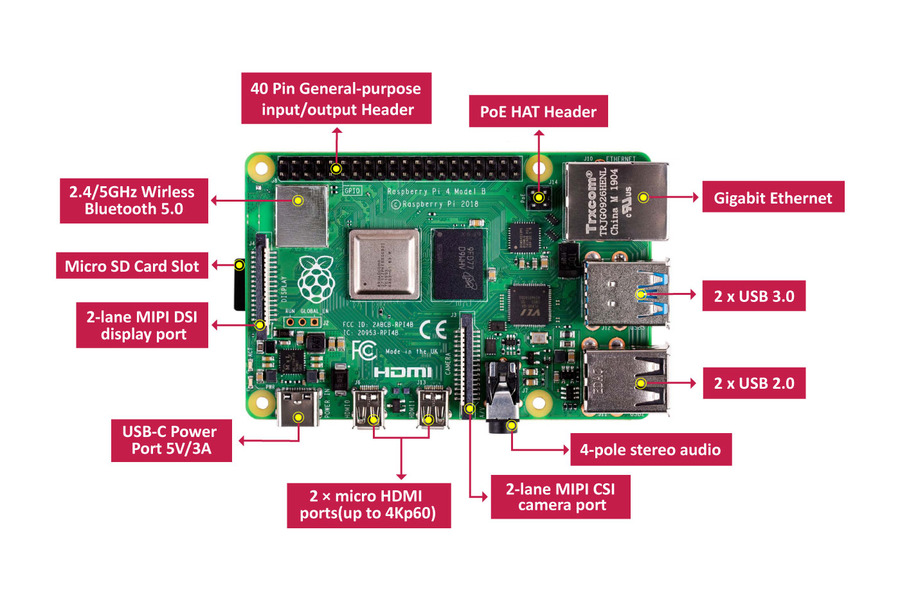
\includegraphics[width=0.5\textwidth]{Rpi}
\caption{Raspberry Pi 4B}\\ 
Source: \textit{https://tinyurl.com/mry6mvjv}
\label{fig:Raspberyypi}
\end{figure}

\section{Relay Module}
\begin{figure}[h]
\centering  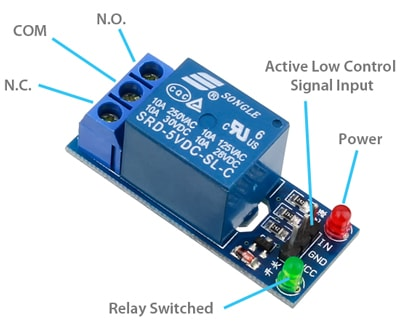
\includegraphics[width=0.4\textwidth]{relay}
\caption{1- Channel Relay}\\ 
Source: \textit{https://tinyurl.com/2356n4m}
\label{fig:Relay}
\end{figure}
Relays are electrically operated switches that open and close circuits.They permit a small amount of electrical current to control high current loads.They protect the control systems from high voltage and currents as they are used to provide electrical isolation between the control and load circuits.

\section{Motor}

\begin{figure}[h]
    \centering

    \begin{minipage}{0.49\textwidth}
        \centering
        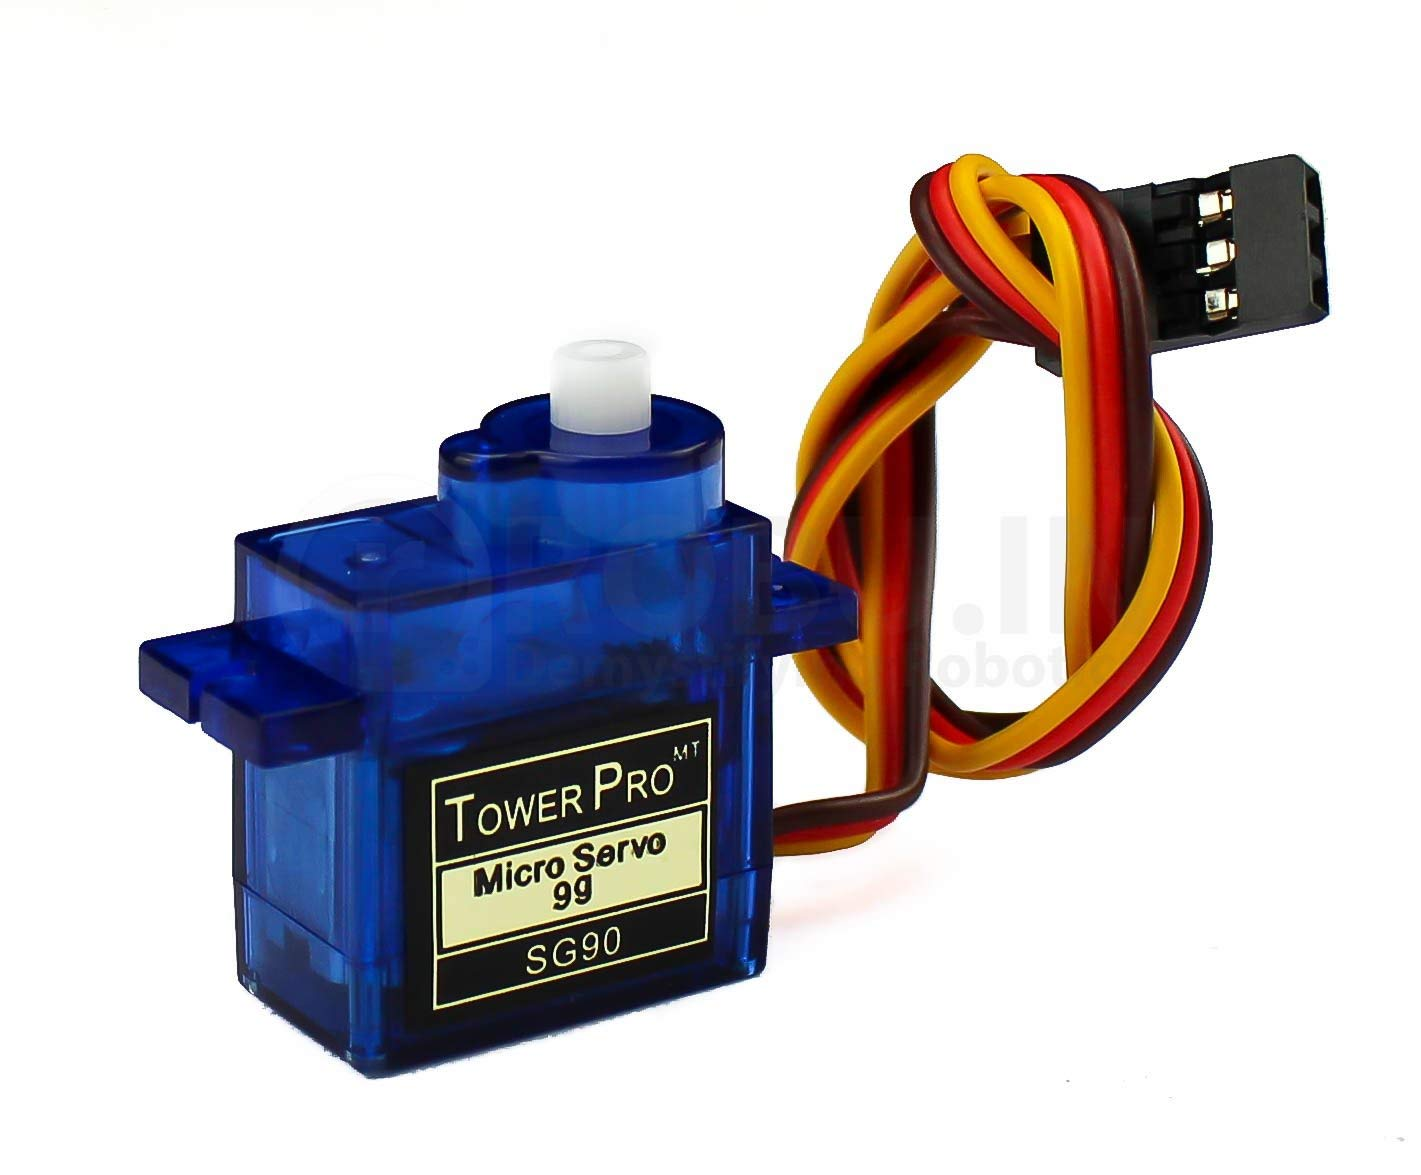
\includegraphics[width=0.5\textwidth]{servo}
        \caption{Servo Motor}\\ 
        Source: \textit{https://tinyurl.com/bdff8n57}
        \label{fig:servo}
    \end{minipage}
    \hfill
    \begin{minipage}{0.49\textwidth}
        \centering
        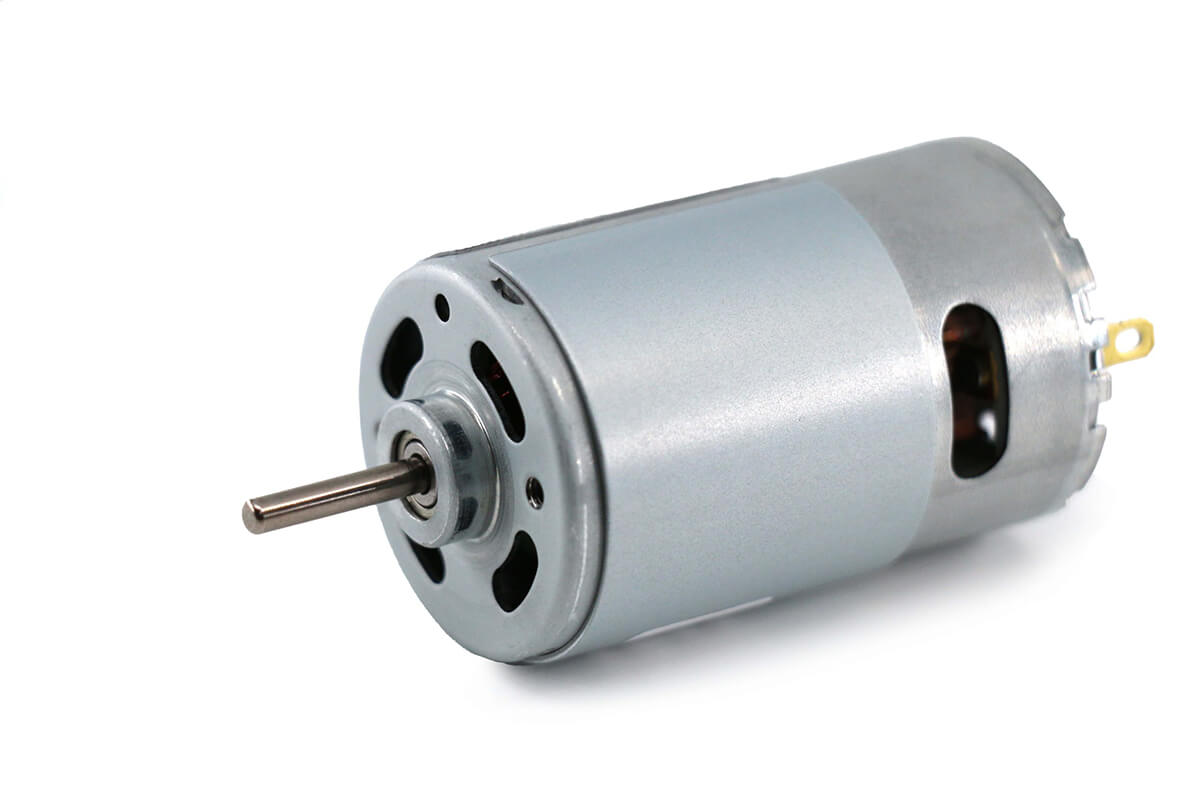
\includegraphics[width=0.5\textwidth]{DC}
        \caption{DC Motor}\\ 
        Source: \textit{https://tinyurl.com/bdcfpbac}
        \label{fig:dc}
    \end{minipage}

\end{figure}
Motors also known as actuators are fundamental components in robotics, providing the necessary actuation, precision, and control for robot movement and manipulation. With the help of motors, the system can be moved to different locations using a precise control system in the 2D axis. develop your applications. This includes tools to compile your code into native machine code (code for iOS and Android).

\section{Arduino IDE}
The Arduino IDE is a software application designed specifically for programming Arduino boards. It provides users with a convenient and user-friendly interface for writing, editing, and uploading code to Arduino microcontrollers.

\section{PyTorch}
PyTorch is a widely used open-source machine learning framework developed by Facebook's AI Research lab (FAIR). It is known for its flexibility, ease of use, and dynamic computation graph, which makes it particularly well-suited for research and experimentation in deep learning.
It's key features include:
\begin{itemize}
        %define spacing
        \setlength\itemsep{1.5pt}
        %Add items
          \item Tensor Computation
          \item Dynamic Computational Graph
          \item Automatic Differentiation
          \item GPU acceleration 
        \end{itemize}
\section{React.js}
React is a free and open-source front-end JavaScript library for building user interfaces based on components. It can be used to develop single-page, mobile, or server-rendered applications with frameworks like Next.js. It allows the creation of interactive and visually appealing user interfaces. Developers can design and implement components that display real-time status of the appliances.
\section{Express.js}
Express is a back-end web application framework for building RESTful APIs with Node.js, released as open-source software. Express is the back-end component of popular development stacks like the MEAN, MERN or MEVN stack together with the MongoDb database software and a JavaScript front-end framework.

\section{Recurrent Neural Network}
A unique kind of artificial neural network called RNN is designed to cope with time series data or data that contains sequences. RNN are equipped with the idea of ”memory,” which enables them to store the states or details of earlier inputs in order to produce the next output in the sequence.Here, the query data are also the kind of sequence data which needs to be processed to extract feature using the special kind of RNN methods called LSTM. RNNs have been used to generate mathematical proofs and translate human thoughts into words.

\section{Transformer}
The drawbacks of RNN being inability to generalize to long sequences, unparalizability are solved by Transformer. Transformers are used in state of the art in almost all NLP tasks. A transformer is a deep learning model that uses sequential data analysis for understanding and learning the context. It follows encoder-decoder structure and process the entire sequence at a time as shown in \ref{fig:attention}. The encoder of the Transformer processes the input embedding and generate the hidden representations. The input embedding are added with a positional encoding to indicate its position in the sequence before it is fed to the encoder. Self-attention is used to output the attended features which are simply a weighted average of the input features. The attended features signify a combination of most important features related to another feature. Then a normalization and feed forward network is used to transform the attended features to required dimension.
The decoder takes in the hidden representation from encoder and performs cross attention to generate the output sequence. The output generated also depends on the previously generated output of decoder which is initially empty. The rest of the architecture is similar to that of an encoder. The token with the highest probability is chosen to generate the output sequence \cite{a2018_11}.

\begin{figure}[h]
    \centering
    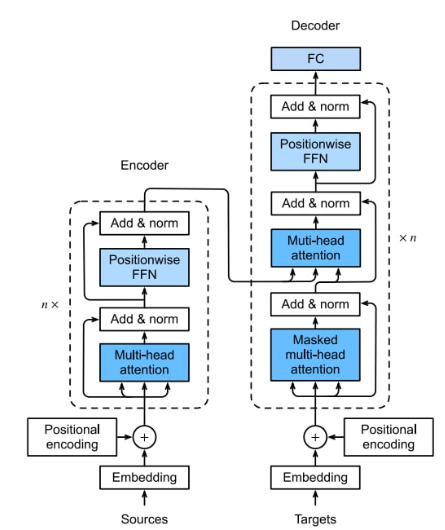
\includegraphics[width=0.8\textwidth]{attention.png}
    \caption{Attention Mechanism}
    \label{fig:attention}
\end{figure}

\section{Whisper}
Whisper is an automatic speech recognition (ASR) system trained on 680,000 hours of multilingual and multitask supervised data collected from the web. We show that the use of such a large and diverse dataset leads to improved robustness to accents, background noise and technical language. The Whisper architecture is a simple end-to-end approach, implemented as an encoder-decoder Transformer. Input audio is split into 30-second chunks, converted into a log-Mel spectrogram, and then passed into an encoder. A decoder is trained to predict the corresponding text caption, intermixed with special tokens that direct the single model to perform tasks such as language identification, phrase-level timestamps, multilingual speech transcription, and to-English speech translation.Other existing approaches frequently use smaller, more closely paired audio-text training datasets or use broad but unsupervised audio pretraining. Because Whisper was trained on a large and diverse dataset and was not fine-tuned to any specific one, it does not beat models that specialize in LibriSpeech performance, a famously competitive benchmark in speech recognition. However, when   Whisper’s zero-shot performance across many diverse datasets was measured , it turns out to  much more robust and makes 50\% fewer errors than other models \cite{a2022_introducing}.

\begin{figure}[h]
    \centering
    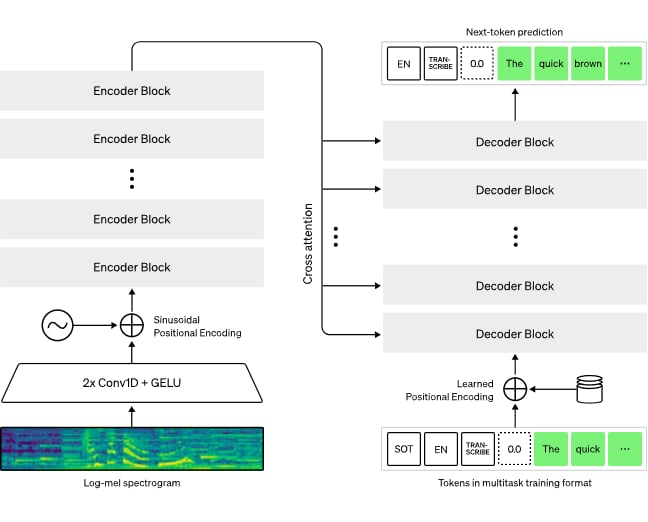
\includegraphics[width=0.8\textwidth]{whisper.jpeg}
    \caption{Architecture of Whisper}
    \label{fig:whisper}
\end{figure}

\newpage